\chapter{Literature Review} 
Artificial Intelligence (AI) is one of the most researched topic in the domain of Computer Science. It is the artificial creation of human-like intelligence that can learn, perceive and process information. AI provides a powerful tool for solving image recognition, document classification as well as for the advancement of interdisciplinary problems. AI is an interdisciplinary domain that make use of various mathematical models, statistical models, neural networks etc to learn pattern and predict unseen data with comparable accuracy. Unlike traditional model, they learn the concepts and rules by learning from examples. Traditional model requires rules to be specified, that results in higher computation but higher accuracy. The ability of AI to generalize even accounting for noise with higher speed promoted various levels of growth, especially in the field of image processing.

Image processing is an interesting field of study that involves image classification, object detection, instance segmentation, object tracking etc. There have been various research and study \cite{diff_algo} to overcome the traditional image processing that employ various algorithm using opencv. Various level of optimization was performed to build deep neural networks that can effectively extract relevant features to identify the object.

\section{Vehicle Identification Systems}
AI have always found it way in developing intelligent system in automobile industry. They are used for smarter manufacturing process, leading to design of efficient systems. They have also helped in business by recommending most efficient path in road network. They are also utilized to build intelligent autonomous vehicles that can react to changes in real-time environment and make way to its destination safely. AI is also used for monitoring purposes for enhancing security. Several parallel papers and researches are build developing such monitoring system using camera network. Below presented are few of such system that are deployed in selected area.

\subsection{CityFlow}
Urban traffic optimization using traffic cameras as sensors is driving the need to advance state-of-the-art multitarget multi-camera (MTMC) tracking. This work  introduces CityFlow \cite{Tang_2019_CVPR}, a city-scale traffic camera dataset having the largest-scale dataset in terms of spatial coverage and the number of cameras/videos in an urban environment. The dataset contains a wide range of scenes, viewing angles, vehicle models, and urban traffic flow conditions. Camera geometry and calibration information are provided to aid spatio-temporal analysis. In addition, a subset of the benchmark is made available for the task of image-based vehicle re-identification (ReID). It also opens a way for new research problems such as vehicle pose estimation, viewpoint generation, etc.

It have compared and bench-marked several state-of-the-art models using Muiti-Target-Single-Camera and Multi-Target-Multi-Camera tracking. They have given emphasis on the visual-spacio-temporal reasoning to re-identification. This approach was able to product better and faster results, handle large scale recognition and is successful in conducting small predictions. However, they require multiple camera scanning same object at multi viewpoint at the same time. It also demanded high quality videos and was also set-up at junction points.

\subsection{Vehicle Make and Model Recognition system}
A Vehicle Make and Model Recognition (VMMR) system \cite{manzoor2019real} can provide great value in terms of
vehicle monitoring and identification based on vehicle appearance in addition to the vehicles attached license plate typical recognition. A VMMR system has a unique set of challenges and issues. Few of the challenges are image acquisition, variations in illuminations and weather, occlusions, shadows, reflections, large variety of vehicles, inter-class and intra-class similarities, addition/deletion of vehicles models over time, etc. The system extract image features from vehicle images and create feature vectors to represent the dataset. Then, two classification algorithms, Random Forest (RF) and Support Vector Machine (SVM) are used for classification. The proposed VMMR system recognizes vehicles on the basis of make, model, and generation (manufacturing years).

For feature extraction, HOG and GIST algorithm are utilized. These vectors are saved in database supporting faster processing speed and improved recognition accuracy, accounting for partial viewpoints. However they have limited region interest with high computation time with increase in block of HOG. The system only addresses local high dimensional features, and have no global representation.

\subsection{Multi-level Feature extraction}
The intelligent transportation system is currently an active research area, and vehicle
re-identification (Re-Id) is a fundamental task to implement it. It determines whether the given vehicle image obtained from one camera has already appeared over a camera network or not. This task becomes more challenging because of intra-class similarity,
viewpoint changes, and inconsistent environmental conditions. A system \cite{cai2019efficient} is proposed which re-identifies a vehicle in two steps: first, shortlist the vehicle from a gallery set on the basis of appearance, and then in the second step, verify the shortlisted vehicle’s license plates with a query image to identify the targeted vehicle. 

The global channel extracts the feature vector from the whole vehicle image, and the local region channel extracts more discriminative and salient features from different regions. A Siamese neural network is used to verify license plates to reach the
exact vehicle. The system also account for color, model, and type as parameters of feature vectors. However, a significant impact of illumination can be found, which is worsen by background clutter. It also do not account for cross camera vehicle tracking.

\subsection{Trends in Vehicle Re-Identification}
Vehicle Re-identification (re-id) over surveillance camera network with non-overlapping
field of view is an exciting and challenging task in intelligent transportation systems (ITS). Vehicle re-id matches targeted vehicle over non-overlapping views in multiple camera network. However, it becomes more difficult due to inter-class similarity, intra-class variability, viewpoint changes, and spatio-temporal uncertainty. In order to draw a detailed picture of vehicle re-id research, this research \cite{deng2021trends} provides a comprehensive description of the various vehicle re-id technologies, applicability, datasets, and a brief comparison of different methodologies. 
This research specifically focuses on vision-based vehicle re-id approaches, including vehicle appearance, license plate, and spatio-temporal characteristics. Some of the main technology taken under consideration are:
\begin{enumerate}
	\item Magnetic Sensor-Based Vehicle Re-Identification
	\item Inductive Loop-Based Vehicle Re-Identification
	\item Global Positioning Systems-Based Vehicle Re-Identification
	\item Vision-Based Vehicle Re-Identification
	\begin{enumerate}
		\item Feature Representation for Vehicle Re-Identification
		\item Traditional Machine Learning-Based Vehicle Re-Identification
		\item Similarity Metric for Vehicle Re-Identification
		\item Fine-Grained Visual Recognition-Based Vehicle Re-Identification
		\item View-Aware-Based Vehicle Re-Identification
		\item Generative Adversarial Network-Based Vehicle Re-Identification
		\item Attention Mechanism
		\item License Plate-Based Vehicle Re-Identification
	\end{enumerate}
	\item Spatio-Temporal Cues-Based Vehicle Re-Identification Approaches
	\item Hybrid Methods-Based Vehicle Re-Identification
\end{enumerate}


\section{Traditional Methods of Image processing}
Traditional methods are computation intensive and hence slow. However, they have higher accuracy, but prone to noise. Some of the methods are:
\begin{enumerate}
	\item Harris Algorithm \\
			Corner detection algorithm that identifies and compares the corners of objects and then compute the similarity.
	\item SIFT: Scale Invariant Feature Transform\\
			Key-points of objects are first extracted from a set of reference images[1] and stored in a database. An object is recognized in a new image by individually comparing each feature from the new image to this database and finding candidate matching features based on Euclidean distance of their feature vectors. 
	\item HOG: Histogram of Oriented Gradients \\
			It counts occurrences of gradient orientation in localized portions of an image, computed on a dense grid of uniformly spaced cells and uses overlapping local contrast normalization for improved accuracy.
	\item GLOH: Gradient Location and Orientation Histogram \\
			It is a SIFT-like descriptor that considers more spatial regions for the histograms. An intermediate vector is computed from Location and orientation bins, for different dimensions.
	\item Canny Edge detection \\
		It is a technique to extract useful structural information from different vision objects and dramatically reduce the amount of data to be processed.
	\item SURF: Speed-ed Up Robust Features \\
			It is a fast and robust algorithm for local, similarity invariant representation and comparison of images. The main interest of the SURF approach lies in its fast computation of operators using box filters, thus enabling real-time applications such as tracking and object recognition. 
	\item DPM: Deformable Parts Model \\
			Special case of Dalal and Triggs Detector, making improvement over HOG and Support Vector Machine (SVM). Figure \ref{fig:dpm} shows the steps for detection of human.
\end{enumerate} 


\begin{figure}[!h]
	\centering
	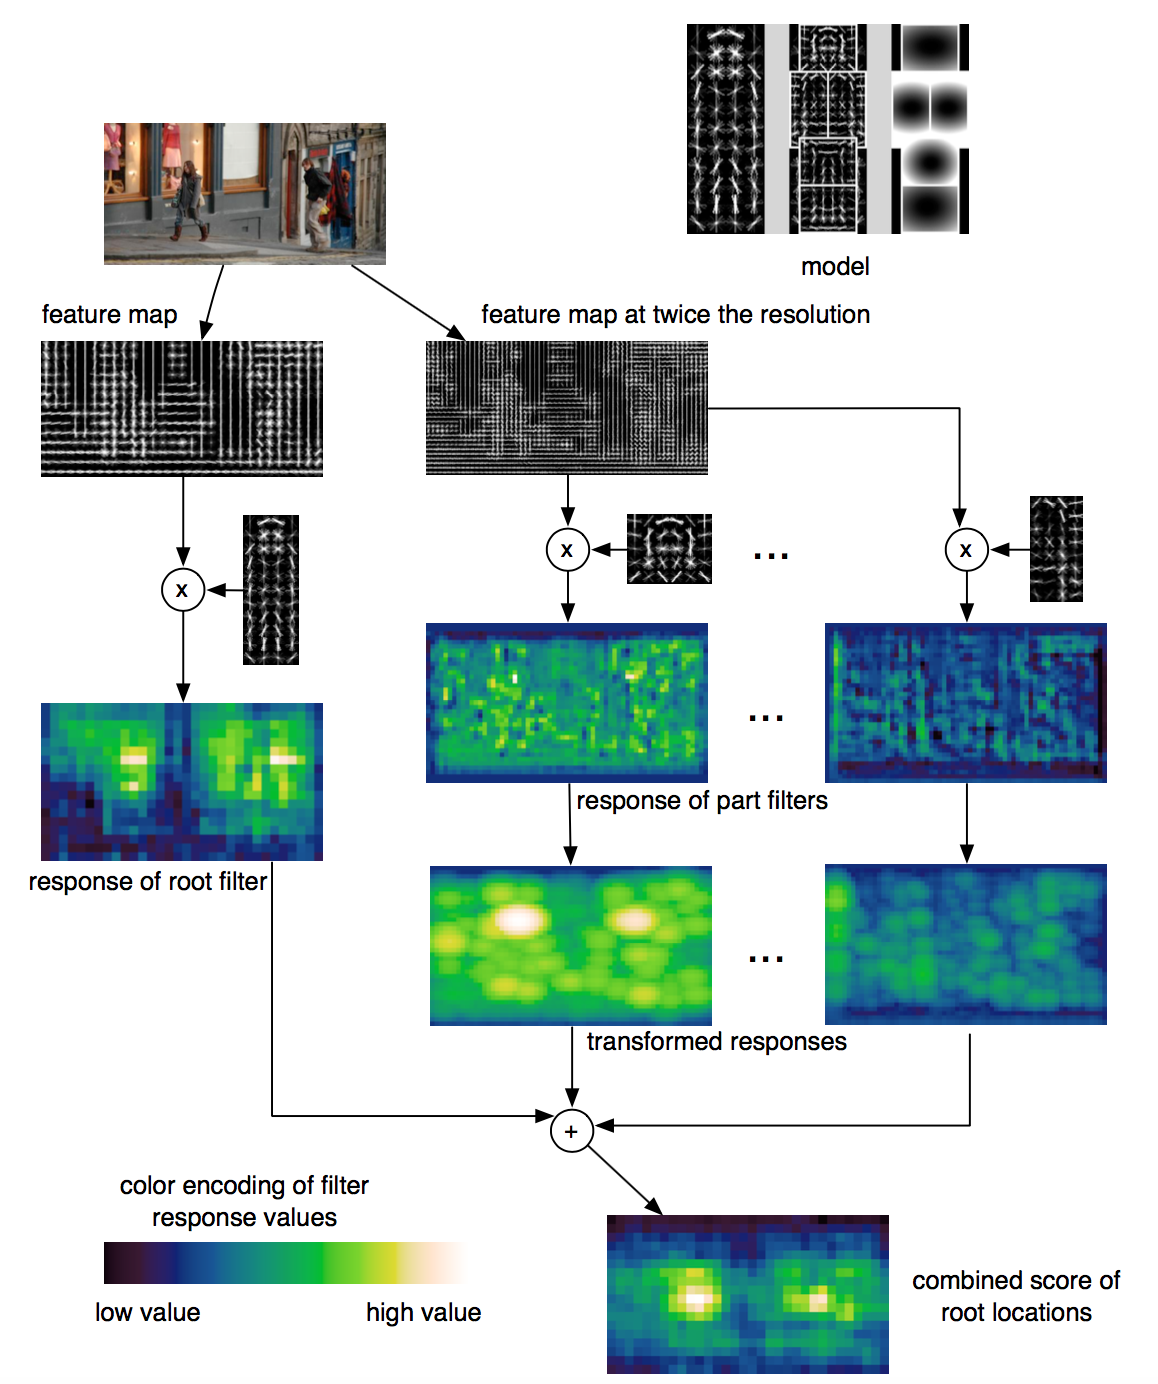
\includegraphics[height=0.5\textheight]{Images/DPM}
	\caption{Deformable Parts Model for Human detection}
	\label{fig:dpm}
	%SRC: https://github.com/lilianweng/lilianweng.github.io/blob/master/posts/2017-12-15-object-recognition-part-2/DPM-matching.png

\end{figure}

\section{Neural Network Models}
Neural Network model consists of neurons firing signals to change the output. Each neuron have weights associated along with activation function. The learning happens through the change of each weights. They require higher training time, but produce output faster along with the ability to resist the effect of noise. They generalize well event to identify occluded objects from image. 

The major jump from traditional method into network model was on to the introduction of AlexNet Model. AlexNet have 5 convolution layers that effectively scale and extract the features. They are then pooled at each layers. At the end, a dense neural network gets trained to predict values for the output neuron, which are softmax-ed to obtain particular class. Dense neural network mimics a classifier. They are used for image classification. To account for various dimension of image, a concept of image pyramid is used to process image at various levels. VGG is an extension of AlexNet. Figure \ref{fig:alexnet_vgg} shows the architecture of AlexNet and VGG model. Convolutional Neural Network (CNN) is a set of filters that extract a specific feature by applying some kernel.

\begin{figure}[h!]
	\centering
	\begin{tabular}[!ht]{m{0.4\hsize}m{0.55\hsize}}
		\begin{subfigure}[b]{\linewidth}
			\centering
			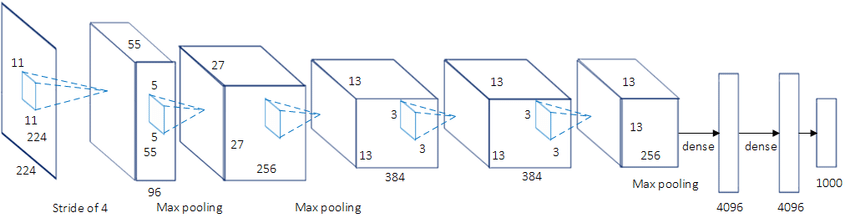
\includegraphics[width=0.9\linewidth]{Images/AlexNet_3D}
			\caption{AlexNet Architecture}
			% SRC: https://www.researchgate.net/figure/AlexNet-Convolutional-Neural-Network-architecture-Figure-reproduced-from-14_fig1_316450908
		\end{subfigure}
		
		\begin{subfigure}[b]{\linewidth}
			\centering
			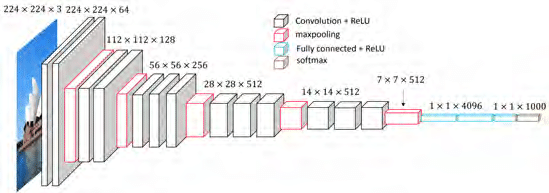
\includegraphics[width=0.9\linewidth]{Images/VGG_3D}
			\caption{VGG Architecture}
			% SRC: https://www.researchgate.net/figure/The-architecture-of-a-VGGNet-CNN-after-Wang-et-al-2017_fig1_323796590
		\end{subfigure}
	
		& 
		\begin{subfigure}[b]{\linewidth}
			\centering
			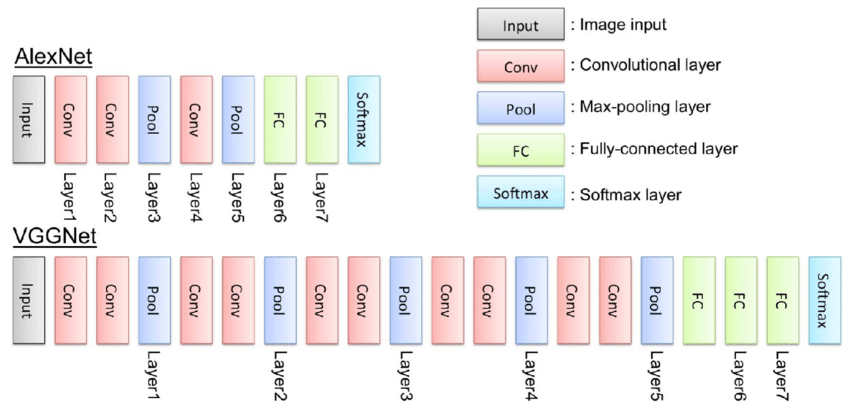
\includegraphics[width=\linewidth]{Images/AlexNet-and-VGGNet-architecture}
			\caption{Layers of model. Classification done by FC layers}
			%SRC: https://www.researchgate.net/figure/AlexNet-and-VGGNet-architecture_fig1_282270749
		\end{subfigure}
	\end{tabular}
	\caption{AlexNet \& VGG Model}	
	\label{fig:alexnet_vgg}
\end{figure}

Owing to the success of AlexNet and VGG model, various study and research are conducted on the CNN layers to efficiently extract features. Some of the major contributions are summarized below.

\subsubsection{Overfeat}
\begin{itemize}
	\item Problem addressed
		\begin{itemize}
			\item CNN network can accept only fixed size images. To process a large image, the image needs to be cropped and resized to fit the dimension of the input of the network. The size constraint is imposed not because of the input layers, but due to the FC layers.
			\item One solution involves manually cropping the image and feeding the network, a stimulation of sliding window. It involves redundant calculation at the image pixels.
		\end{itemize}
	\item Solution Proposed
		\begin{itemize}
			\item Implementation of FC as Conv network, removing the input constraint
			\item Image pyramid of 6 sizes [ 461*569 , 425*497 , 386*461 , 317*389 , 281*317 , 245*245 ] creating spatial output dimensions. The spacial output dimensions show how many object can be detected from the image
		\end{itemize}
\end{itemize}

\begin{figure}[h!]
	\centering
	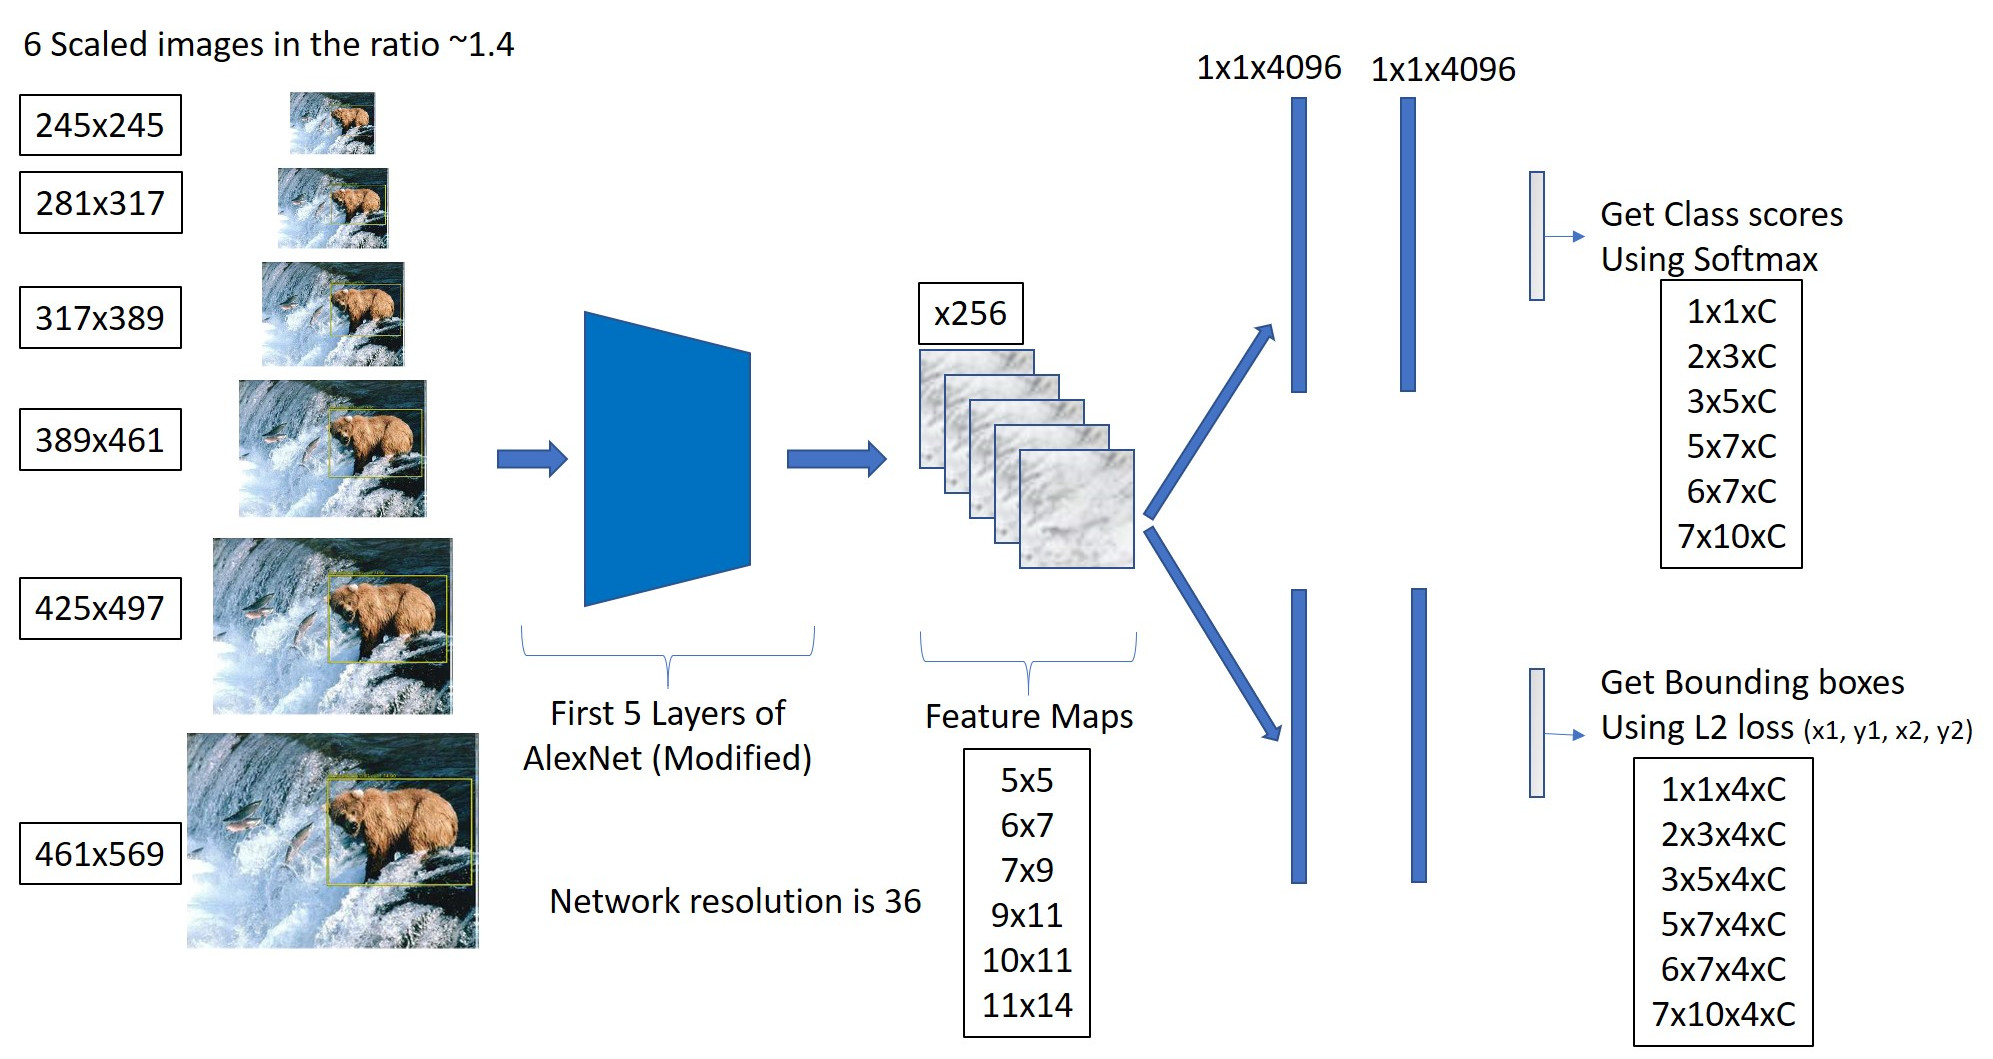
\includegraphics[width=0.9\linewidth]{Images/overfeat}
	\caption{Overfeat Architecture}
	%SRC: https://cogneethi.com/assets/images/evodn/detection_overfeata_detect.jpg
\end{figure}

\subsubsection{R-CNN: Regions with Convolutional Neural Networks}
%SRC: https://towardsdatascience.com/r-cnn-fast-r-cnn-faster-r-cnn-yolo-object-detection-algorithms-36d53571365e
To bypass the problem of selecting a huge number of regions, we can use selective search to extract just 2000 regions from the image - called region proposals. These 2000 region proposals are generated using the selective search algorithm. These 2000 candidate region proposals are warped into a square and fed into a convolutional neural network that produces a 4096-dimensional feature vector as output. The CNN acts as a feature extractor and the output dense layer consists of the features extracted from the image and the extracted features are fed into an SVM to classify the presence of the object within that candidate region proposal. The algorithm also predicts four values which are offset values to increase the precision of the bounding box. Some of the drawbacks are
\begin{itemize}
	\item It still takes a huge amount of time to train the network as we would have to classify 2000 region proposals per image.
	\item It cannot be implemented real time as it takes around 47 seconds for each test image.
	\item The selective search algorithm is a fixed algorithm. Therefore, no learning is happening at that stage. This could lead to the generation of bad candidate region proposals.
\end{itemize}

\begin{figure}[h!]
	\centering
	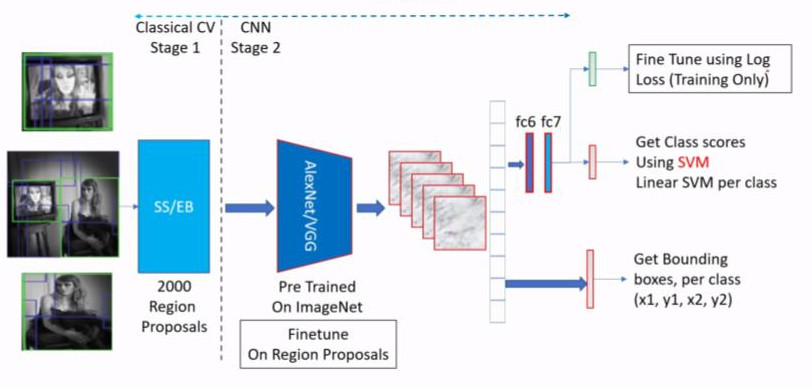
\includegraphics[width=0.9\linewidth]{Images/RCNN}
	\caption{R-CNN model}
	\label{fig:rcnn}
\end{figure}

The same author of the previous paper(R-CNN) solved some of the drawbacks of R-CNN to build a faster object detection algorithm and it was called \textbf{Fast R-CNN}. The approach is similar to the R-CNN algorithm. But, instead of feeding the region proposals to the CNN, we feed the input image to the CNN to generate a convolutional feature map. From the convolutional feature map, we identify the region of proposals and warp them into squares and by using a RoI pooling layer we reshape them into a fixed size. From the RoI feature vector, softmax layer is used to predict the class of the proposed region and also the offset values for the bounding box. “Fast R-CNN” is faster than R-CNN is because we do not need to feed 2000 region proposals to the CNN every time. Instead, the convolution operation is done only once per image and a feature map is generated from it.

Both of the above algorithms(R-CNN \& Fast R-CNN) uses selective search to find out the region proposals. Selective search is a slow and time-consuming process affecting the performance of the network. Therefore an object detection algorithm was proposed in \textbf{Faster-RCNN} that eliminates the selective search algorithm and lets the network learn the region proposals. Similar to Fast R-CNN, the image is provided as an input to a convolutional network which provides a convolutional feature map. Instead of using selective search algorithm on the feature map to identify the region proposals, a separate network is used to predict the region proposals. The predicted region proposals are then reshaped using a RoI pooling layer which is then used to classify the image within the proposed region and predict the offset values for the bounding boxes.

\subsection{YOLO: You Only Look Once}
YOLO \cite{yolo_core_paper} is a clever CNN for doing object detection in real-time. The algorithm applies a single neural network to the full image, and then divides the image into regions and predicts bounding boxes and probabilities for each region. These bounding boxes are weighted by the predicted probabilities. The algorithm “only looks once” at the image in the sense that it requires only one forward propagation pass through the neural network to make predictions. After non-max suppression it then outputs recognized objects together with the bounding boxes. With YOLO, a single CNN simultaneously predicts multiple bounding boxes and class probabilities for those boxes. YOLO trains on full images and directly optimizes detection performance. 

\subsubsection{Steps}
\begin{enumerate}
	\item YOLO is based on the idea of segmenting an image into smaller images. The image is split into a square grid of dimensions $S*S$. The cell in which the center of an object resides, is the cell responsible for detecting that object. 
	
	\item Each cell will predict $B$ bounding boxes and a confidence score for each box. Each of these bounding boxes is made up of 5 numbers: the x position, the y position, the width, the height, and the confidence. 
	
	\item The coordinates $(x, y)$ represent the location of the center of the predicted bounding box, and the width and height are fractions relative to the entire image size. The confidence represents the Intersection Over Union (IOU) between the predicted bounding box and the actual bounding box, referred to as the ground truth box. 
	
	\item Each cell also predicts the class of the object. This class prediction is represented by a one-hot vector length $C$, the number of classes in the dataset. However, while each cell may predict any number of bounding boxes and confidence scores for those boxes, it only predicts one class. 
	
	\item Each prediction from a grid cell will be of shape $C + B * 5$. Because there are $S*S$ grid cells in each image, the overall prediction of the model is a tensor of shape $S*S*(C+B*5)$.
\end{enumerate}
\begin{figure}[h!]
	\centering
	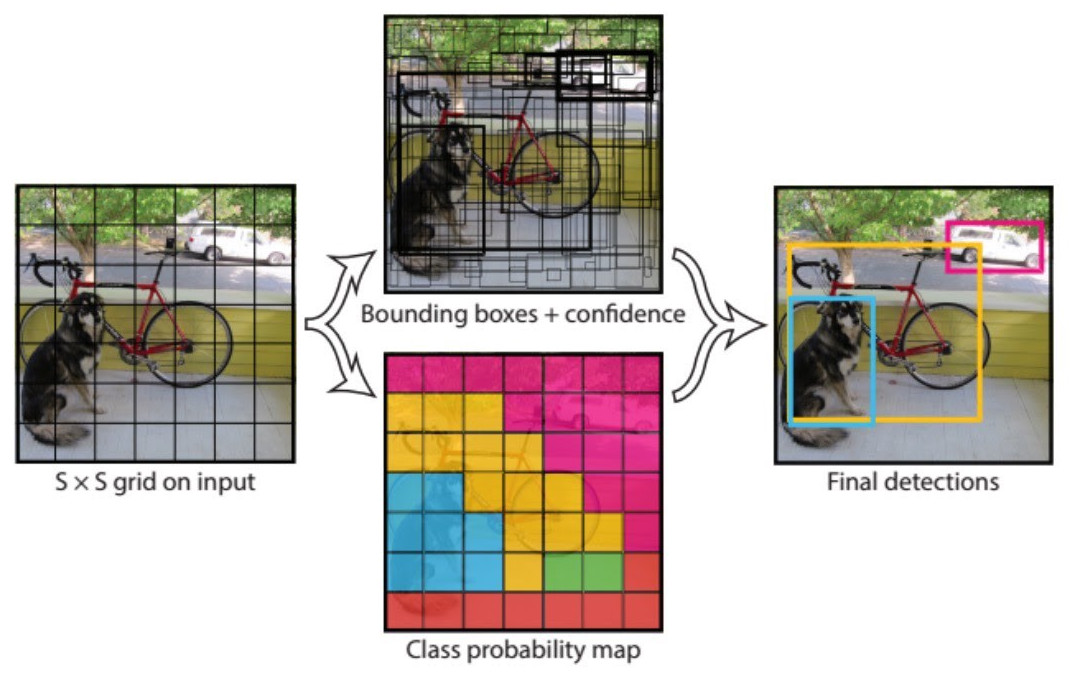
\includegraphics[width=0.7\linewidth]{Images/yolo_steps}
	\caption{YOLO detection steps}
	%SRC: https://towardsdatascience.com/evolution-of-yolo-yolo-version-1-afb8af302bd2
\end{figure}

\subsubsection{Architecture}
The YOLO model is made up of three key components:
\begin{enumerate}
	\item The Backbone \\
	It is the part of the network made up of convolutional layers to detect key features of an image and process them. The backbone is first trained on a classification dataset and typically trained at a lower resolution than the final detection model, as detection requires finer details than classification. YOLOv4 have CSP-Darknet-53 as the backbone of the network 

	\item The Neck \\
	It uses the features from the convolution layers in the backbone with fully connected layers to make predictions on probabilities and bounding box coordinates. 
	
	\item The Head \\
	It is the final output layer of the network which can be interchanged with other layers with the same input shape for transfer learning. 	
\end{enumerate} 
These three portions of the model work together to first extract key visual features from the image then classify and bound them. This happens for multiple scales. Each YOLO head corresponds to particular scale of detection. They are the combined on score values to produce final detection. Figure \ref{fig:yolov4-architecture} shows the architecture of YOLOv4 model.

\begin{figure}[H]
	\centering
	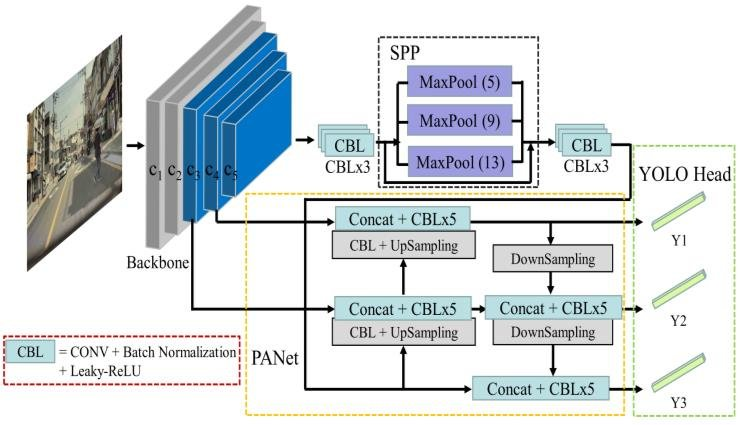
\includegraphics[width=0.85\linewidth]{Images/YOLOV4-research-gate}
	\caption{YOLOv4 architecture}
	\label{fig:yolov4-architecture}
	%SRC: https://www.researchgate.net/figure/Overall-structure-of-YOLOv4-including-CSPDarknet-backbone-SPPnet-PANet-and-3-YOLO_fig2_344919620
\end{figure}


\subsubsection{YOLO variants}
\begin{table}[H]
	\centering
	\begin{tabular}{|c|c|c|c|c|}
		\hline
		\textbf{Variant} & \textbf{Release} & \textbf{FPS} & \textbf{mAP} & \textbf{Feature Extractor} \\ \hline
		\begin{tabular}[c]{@{}c@{}}YOLOv1\\ (448*448)\end{tabular} & \begin{tabular}[c]{@{}c@{}}6 May 2016\\ Joseph Redmon\end{tabular} & 45 & 63.4 & \begin{tabular}[c]{@{}c@{}}24 CNN\\ 2 FC\end{tabular} \\ \hline
		\begin{tabular}[c]{@{}c@{}}YOLOv2\\ (416*416)\end{tabular} & \begin{tabular}[c]{@{}c@{}}25 Dec 2016\\ Joseph Redmon\end{tabular} & 67 & 76.8 & VGG-16 \\ \hline
		\begin{tabular}[c]{@{}c@{}}YOLOv3\\ (416*416)\end{tabular} & \begin{tabular}[c]{@{}c@{}}8 April 2018\\ Joseph Redmon\end{tabular} & 35 & 55.3 & Darknet-53 \\ \hline
		\begin{tabular}[c]{@{}c@{}}YOLOv4\\ (416*416)\end{tabular} & \begin{tabular}[c]{@{}c@{}}23 April 2020\\ Alexey Brochkovskiy\end{tabular} & 38 & 62.8 & CSPDarknet-53 \\ \hline
		YOLOv5 & \begin{tabular}[c]{@{}c@{}}18 May 2020\\ Glenn Jocher\end{tabular} & 70.9 & 66.9 & CSPDarknet-53 \\ \hline
		\begin{tabular}[c]{@{}c@{}}PP-YOLO\\ (416*416)\end{tabular} & \begin{tabular}[c]{@{}c@{}}3 August 2020\\ Xiang Long\end{tabular} & 72.9 & 62.8 & ResNet50-vd-dcn \\ \hline
	\end{tabular}
	\caption{YOLO variants comparison}
\end{table}

\subsection{DeepSORT: SORT with Deep Association}
Simple Online and Realtime Tracking (SORT) \cite{sort} is a pragmatic approach to multiple object tracking with a focus on simple, effective algorithms. DeepSort \cite{deepsort} is an integration to improve the performance of SORT. Due to this extension, we are able to track objects through longer periods of occlusions, effectively reducing the number of identity switches. Much of the computational complexity is spend in learning a deep association metric. During online application, we establish measurement-to-track associations using nearest neighbor queries in visual appearance space. 

Traditional SORT algorithm simply uses the Kalman filter along with Hungarian algorithm for the tracking components. It achieves a speed of 260Hz. Kalman filtering, also known as linear quadratic estimation (LQE), is an algorithm that uses a series of measurements observed over time and produces estimates of unknown variables that tend to be more accurate than those based on a single measurement alone, by estimating a joint probability distribution over the variables for each time frame. The Hungarian method is a combination optimization algorithm that solves the assignment problem in polynomial time and which anticipated later primal–dual methods. It gives a good tracking of object. But the id association fails where object osculation or sudden change in motion happens. It fails when the object is completely covered by another object. A deep association provides better re-identification even after skipping few frames. The feature vectors are matched using cosine distance similarity \cite{deep_cosine}.

\begin{figure}[h!]
	\centering
	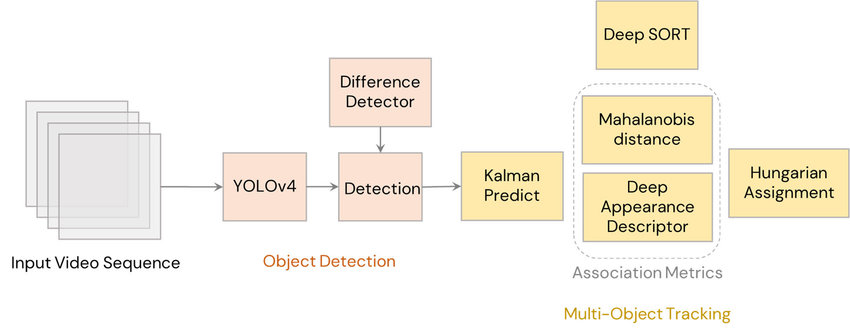
\includegraphics[width=0.8\linewidth]{Images/deepsort}
	\caption{DeepSORT architecture}
	\label{fig:deepsort}
	%SRC: https://www.researchgate.net/figure/Architecture-of-Deep-SORT-Simple-online-and-real-time-tracking-with-deep-association_fig2_353256407
\end{figure}

Figure \ref{fig:deepsort} depicts architecture of DeepSORT. Frames of a series of time-series are passed into image detection model (Here YOLOv4). The model computes the bounding box for each detection. They are passed into a Detection Module to extract the feature vector, also called as 'encoders'. They are passed into Kalman filter for prediction. Cosine similarity is used to associate ID. It is supported by Deep metric (Deep appearance Descriptor) and finally the next location is predicted in polynomial time using Hungarian Assignment technique. Several articles \cite{deepsort_web}  \cite{theaiguyscode_deepsort} and GitHub repository \cite{obj_track_deep_yolo} shows the implementation of Deepsort for Human re-identification.


\subsection{Siamese Network}
A Siamese neural network (also called a twin neural network) is an artificial neural network that uses the same weights while working on two different input vectors to compute comparable output vectors. The are often used for face matching, fingerprint matching, recognizing handwritten checks, and matching queries with indexed documents etc. It have a simple and unique architecture apart form other neural networks as shown in figure \ref{fig:siamese}.

\begin{figure}[h!]
	\centering
	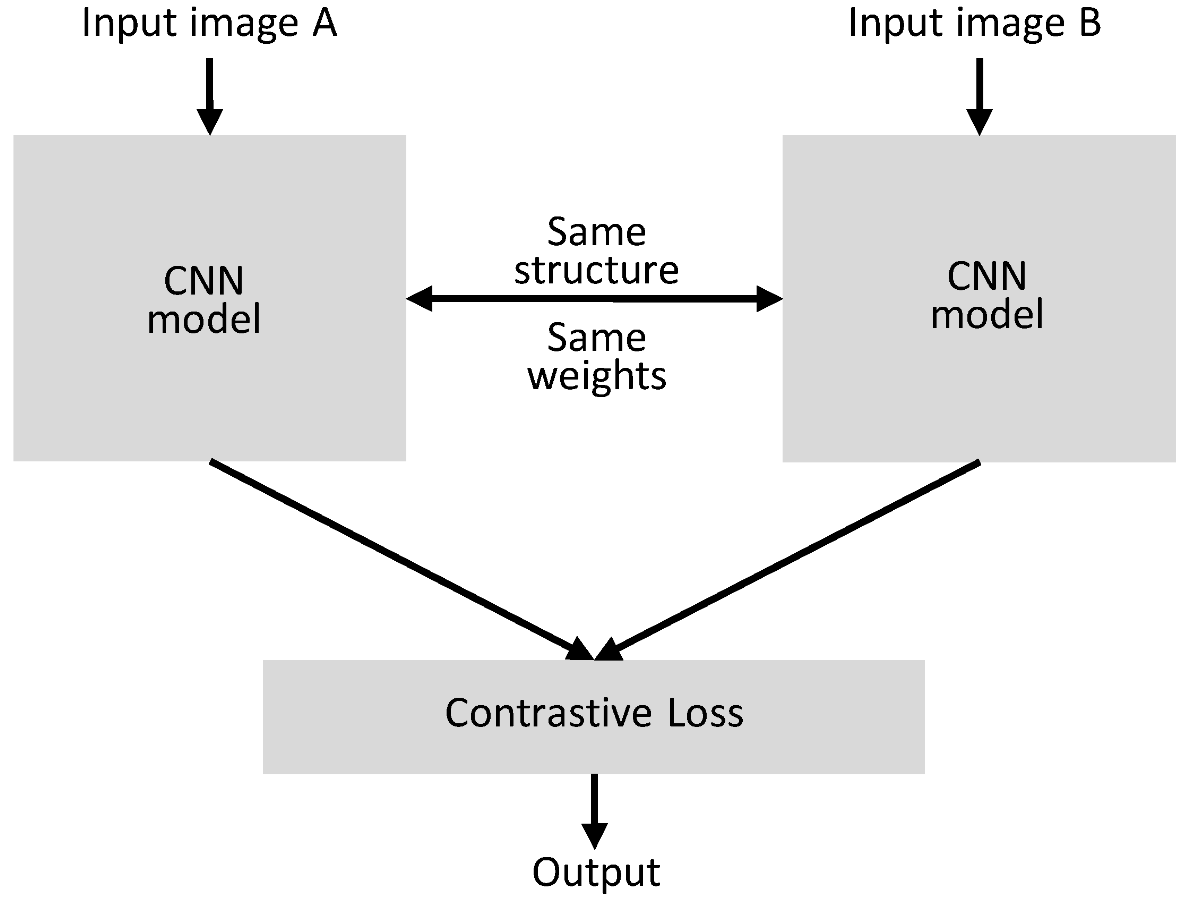
\includegraphics[width=0.5\linewidth]{Images/siamese}
	\caption{Siamese Network architecture}
	\label{fig:siamese}
	%SRC: https://miro.medium.com/max/1400/1*jQcJ7ik58aeTV0As2d9Jcw.png
\end{figure}
 
The network consists of two identical CNN models for feature extraction. The CNN model is trained separately to identify the images. The last classification layer of the separately trained CNN model is remove so that the feature vector is extracted. The feature vector from the two identical CNN model is passed into DNN layer of Siamese network that outputs if the images are similar or not. One of the image is called the anchor image and the other is the test images. Keras article \cite{siamese_keras} and GitHub repository \cite{siamese_git} provides excellent reference materials.


